\section{Introduzione}
Il progetto mira a sfruttare gli alberi di decisione per estrarre in maniera automatica regole di classificazione, con l’obiettivo di identificare file malevoli. Queste regole verranno poi tradotte in un programma ASP (Answer Set Programming) per realizzare un sistema di malware detection. Come base dati è stato scelto il dataset EMBER \cite{ember}, uno dei dataset più noti nel campo dell’analisi dei malware, che fornisce un ampio insieme di campioni malware e benigni per addestrare e validare i modelli predittivi. L’intento del progetto è coniugare la capacità interpretativa degli alberi di decisione con la flessibilità di ASP, così da sviluppare un sistema capace di rilevare e classificare con efficacia i malware, mantenendo al contempo un elevato livello di trasparenza nei processi decisionali.
\subsection{Il formato PE}\label{subsec:pe_format}
Il formato di file PE (Portable Executable) \cite{pe} rappresenta lo standard prevalente per i file eseguibili, librerie a collegamento dinamico (DLL) e driver di dispositivi  nelle versioni a 32-bit e 64-bit del sistema operativo Microsoft Windows.  La struttura del formato PE si basa su una serie di intestazioni standard (si veda la Figura~\ref{fig:pe_header} per il formato PE-32), seguite da una o più sezioni. Tra le intestazioni, quella del formato \textbf{Common Object File Format} (COFF) fornisce diverse informazioni essenziali sul file, come il tipo di macchina a cui è destinato, la sua natura (e.g. eseguibile, DLL, oggetto) o il numero di sezioni e simboli. L'\textbf{intestazione opzionale}, invece, specifica ulteriori dettagli quali la versione del linker, la dimensione del codice e dei dati e l'indirizzo dell'entry point.
Le sezioni del file
 \begin{figure}[H]
	\centering
	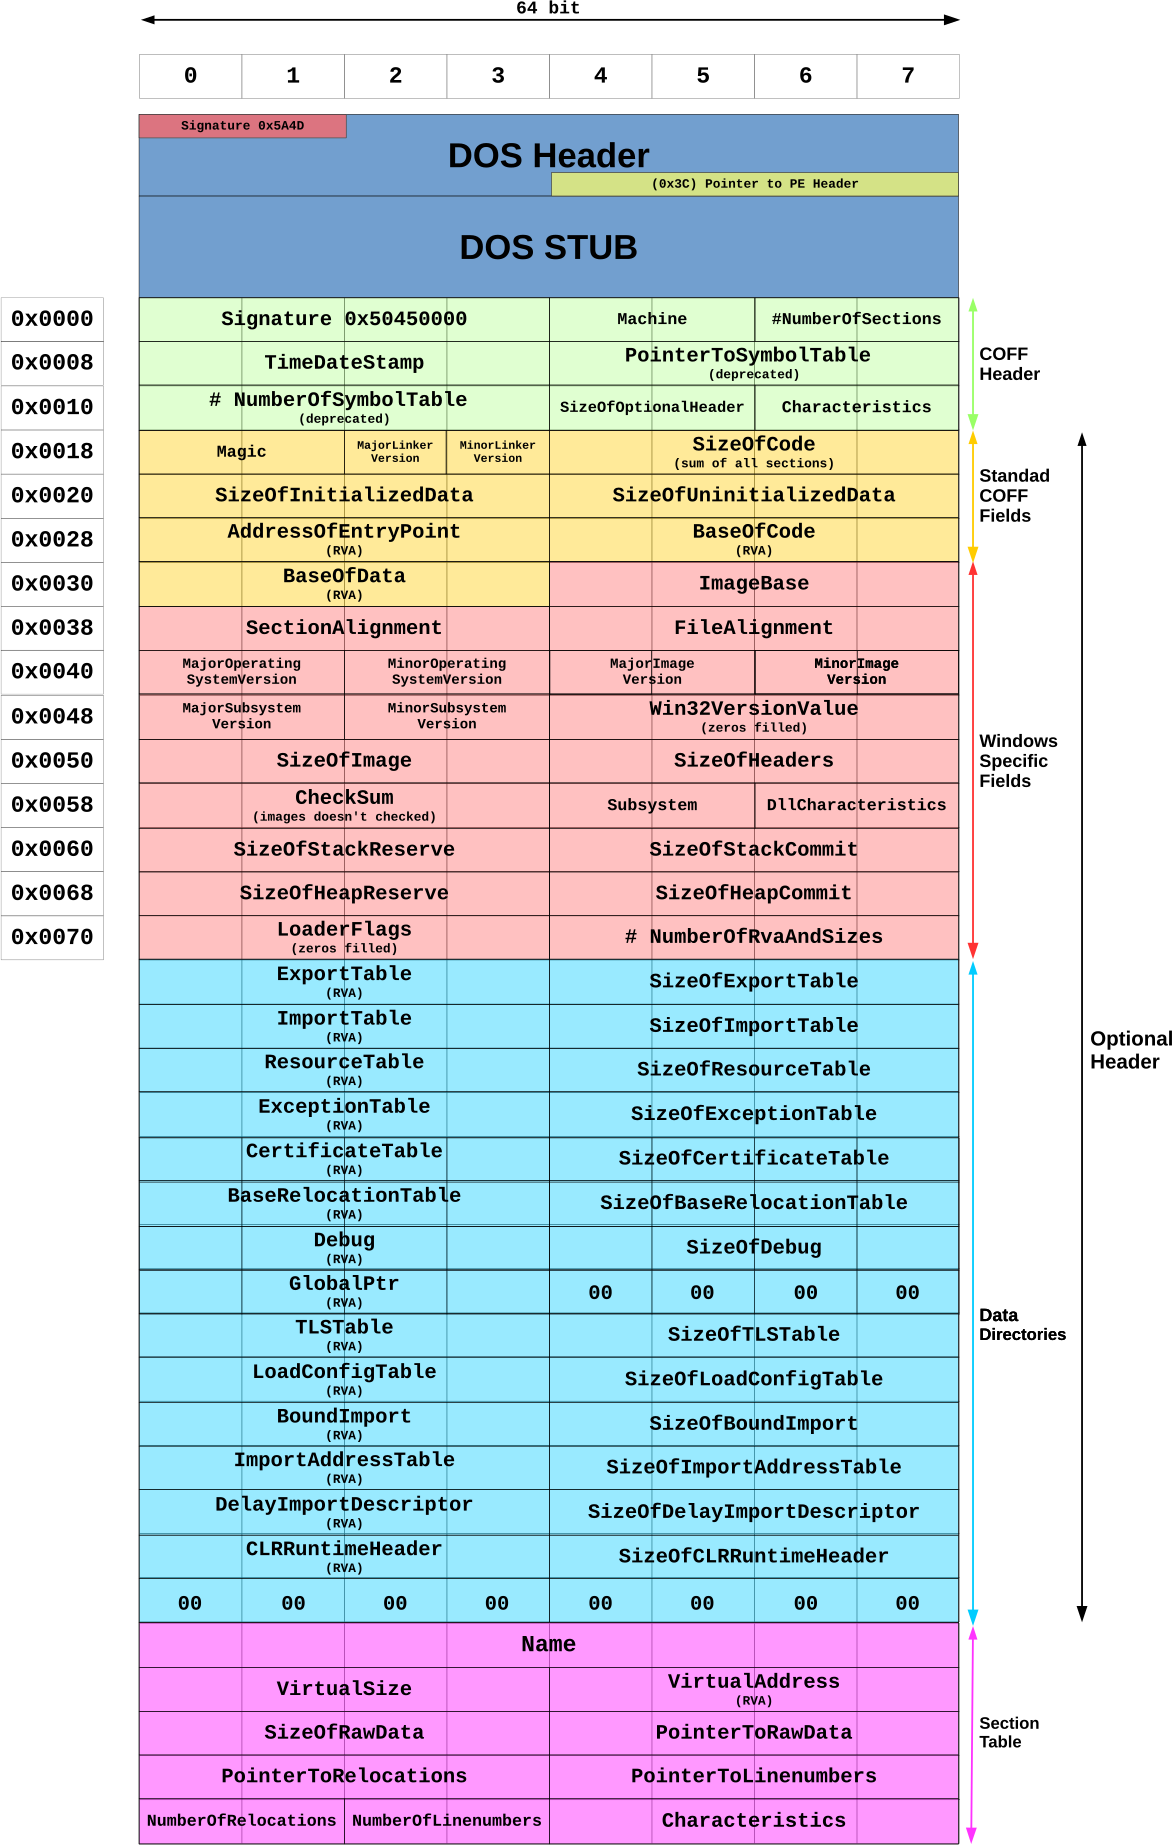
\includegraphics[width=\columnwidth]{fig/pe_format.png}
	\caption{Struttura di un Portable Executable a 32 bit. Creative commons image courtesy \cite{pe_header}}
	\label{fig:pe_header}
\end{figure}
 PE contengono invece il codice e i dati inizializzati, che il loader di Windows deve mappare, rispettivamente, in memoria eseguibile o di lettura/scrittura. Tra queste sezioni, di norma, troviamo: 
\begin{itemize}
    \item \textbf{.text}: Contiene il codice eseguibile del programma.
    \item \textbf{.data}: Memorizza le variabili globali e statiche inizializzate che possono essere modificate durante l'esecuzione del programma.
	\item \textbf{.rdata}: Contiene dati in sola lettura, come le stringhe letterali e le costanti.
    \item \textbf{.bss}: Memorizza dati non inizializzati (\textit{Block Started by Symbol}), come variabili dichiarate ma non inizializzate.
    \item \textbf{.edata}: Contiene informazioni di esportazione, in particolare per le DLL.
    \item \textbf{.idata}: Memorizza informazioni di importazione per funzioni e variabili utilizzate da altri moduli.
    \item \textbf{.reloc}: Memorizza informazioni di rilocazione utilizzate dal \textit{loader} per aggiustare gli indirizzi durante il caricamento dell'eseguibile.
    \item \textbf{.pdata}: Contiene informazioni per la gestione delle eccezioni.
    \item \textbf{.tls}: Sezione \textit{Thread Local Storage}, memorizza dati unici per ciascun thread.
\end{itemize}    
È inoltre possibile aggiungere sezioni personalizzate (ad esempio, la sezione \textbf{.petite} viene creata dal packer \textit{Petite}, uno strumento per comprimere i file PE). In generale, i nomi delle sezioni non hanno vincoli imposti dal loader di Windows, ma spesso seguono convenzioni consolidate. 
\subsection{Il dataset EMBER}
Il dataset Ember, reso pubblico nell'aprile 2018, contiene informazioni su oltre un milione di campioni, suddivisi tra malware e software benigni, rappresentati attraverso un insieme di caratteristiche statiche estratte utilizzando il modulo LIEF \cite{lief}. Questo dataset è costituito da una collezione di file JSON, ognuno dei quali rappresenta le caratteristiche associate a un singolo campione. Le caratteristiche sono suddivise in nove categorie principali, descritte brevemente di seguito:
\begin{itemize}
	\item \textbf{General}. Le caratteristiche incluse sono: dimensione del file, dimensione virtuale del file, numero di funzioni esportate e importate, presenza di informazioni di debug, archivio locale dei thread (\textit{Thread Local Storage}), tabella delle risorse, tabella delle rilocazioni, numero di firme e simboli.
	\item \textbf{Header.} Contiene alcune delle informazioni dell'intestazione (sia COFF che opzionali). L'intestazione COFF contiene il file immagine, la macchina di destinazione e il timestamp, mentre l'intestazione opzionale contiene dettagli sul sottosistema di destinazione, le versioni dell'immagine, la dimensione di commit, l'identificazione del file, la versione della DLL e del linker.
	\item \textbf{Imported.} Contiene una lista di funzioni che sono state importate da librerie a collegamento dinamico.
	\item \textbf{Exported.} Indirizzo, nome e numero di serie dei simboli esportati. La maggior parte dei file EXE non possiede una tabella di esportazione, mentre la maggior parte dei file DLL ne è dotata.
	\item \textbf{Sections.} Contiene informazioni su ogni sezione, inclusi il nome, la dimensione virtuale, la dimensione fisica, l'entropia e l'elenco delle stringhe.
	\item \textbf{Byte Histogram.} Indica il numero di occorrenze di ciascun valore di byte (256 valori interi) nel file PE.
	\item \textbf{Byte Entropy Histogram.} Entropia con finestra di lunghezza fissa, coppie di valori statistici con finestra scorrevole (byte, valore di entropia). In questo caso, la lunghezza della finestra è di 1024 byte, mentre la dimensione del passo è di 256 byte.
	\item \textbf{Strings.} Statistiche semplici sulle stringhe, inclusi istogramma, entropia dei caratteri, lunghezza media, numero di stringhe, percorsi, collegamenti URL, chiavi di registro, ecc.
	\item \textbf{Data Directories.} Tabella delle directory dei dati, che include: tabella delle esportazioni, tabella delle importazioni, directory delle risorse, directory delle eccezioni, directory della sicurezza, tabella delle rilocazioni, directory di debug, informazioni sul copyright, directory dei puntatori, directory TLS, directory della configurazione di caricamento, directory di input per il binding, tabella degli indirizzi di importazione, caricamento ritardato e informazioni COM.
\end{itemize}
I valori delle caratteristiche estratti da ogni programma vengono utilizzati per costruire un vettore di caratteristiche. A ciascun vettore di caratteristiche vengono poi associati tre elementi informativi aggiuntivi: 
\begin{itemize}
	\item L'hash SHA256 del file del file
	\item Il mese e l'anno in cui il file è stato raccolto
	\item Il \textit{ground truth}, ovvero l'etichetta corretta del file (maligno, benigno o non etichettato)
\end{itemize}  
Concludiamo dicendo che il dataset è suddiviso in 900.000 campioni destinati all'addestramento, suddivisi in tre gruppi da 300.000 file ciascuno, uno per ogni classe, e in 200.000 campioni per il test, equamente distribuiti tra malware e file benigni.  È importante sottolineare che i campioni di malware presenti nei dati di test sono più recenti rispetto a quelli dei dati di addestramento, simulando uno scenario reale, in cui i file sconosciuti vengono analizzati utilizzando la conoscenza derivata dai dati storici.
\subsection{Alberi decisionali}\label{subsec:decision_tree}
Gli alberi di decisione sono modelli predittivi spesso utilizzati in problemi di classificazione e regressione, poiché forniscono un modo intuitivo per rappresentare il processo decisionale: si inizia con un nodo radice che corrisponde a una determinata caratteristica del dataset e, attraverso successivi nodi intermedi, si procede ponendo domande o verificando condizioni che permettono di discriminare le istanze in modo sempre più preciso. Il loro funzionamento si basa su un processo ricorsivo, guidato da metriche volte a valutare la purezza dei dati in ciascun nodo: la caratteristica e il criterio di suddivisione selezionati mirano a massimizzare l’omogeneità dei sottogruppi, affinché i nodi che rappresentano la stessa classe (o valori simili, nel caso di regressione) vengano raggruppati in modo efficace. Una delle misure più comuni per valutare tale omogeneità è l’indice di Gini, che calcola la probabilità di estrarre a caso due elementi appartenenti a classi diverse dallo stesso sottoinsieme; valori bassi indicano alta purezza, ovvero istanze che ricadono in una sola classe o in classi molto sbilanciate a favore di una determinata etichetta. L’intero processo continua finché non si raggiungono criteri di arresto come, per esempio, un numero minimo di osservazioni in un nodo oppure quando un ulteriore split non apporterebbe miglioramenti significativi. Per evitare che l’albero si adatti eccessivamente ai dati di addestramento, incorrendo così nell’overfitting, si fa spesso ricorso a tecniche di potatura (pruning) o ad altre forme di regolarizzazione che riducono la complessità del modello pur mantenendo un buon livello di accuratezza. Un ulteriore vantaggio degli alberi di decisione risiede nella loro interpretabilità: il percorso che porta a una determinata previsione risulta chiaro e tracciabile lungo i rami dell’albero, rendendo questi modelli particolarmente adatti in contesti in cui la trasparenza delle decisioni risulta fondamentale.